% =====================================================================
%  醫病共享決策 — 支架（PCI）還是外科繞道手術（CABG）？— Tufte-book 版
%  國立臺灣大學醫學院附設醫院新竹臺大分院 心血管中心．心導管室
%  Engine: XeLaTeX  |  Class: tufte-book
% =====================================================================
\documentclass[justified,nobib,openany]{tufte-book}

% ---------- Fonts (XeLaTeX + xeCJK) ----------
\usepackage{fontspec}
\usepackage{xeCJK}
\setmainfont{ETbb}
\setCJKmainfont[Path=fonts/,BoldFont=NotoSerifTC-Bold.ttf]{NotoSerifTC-Regular.ttf}
\setCJKsansfont[Path=fonts/,BoldFont=NotoSansTC-Bold.ttf]{NotoSansTC-Regular.ttf}
\newCJKfontfamily\hei[Path=fonts/,BoldFont=NotoSansTC-Bold.ttf]{NotoSansTC-Medium.ttf}
\newCJKfontfamily\heibold[Path=fonts/]{NotoSansTC-Bold.ttf}
\setCJKmonofont[Path=fonts/]{NotoSansTC-Regular.ttf}
% 將圈號數字（①②…）歸為 CJK 類，改由 Noto 字型輸出（ETbb 無此字符）
\xeCJKDeclareCharClass{CJK}{"2460 -> "24FF}

% ---------- Packages ----------
\usepackage{graphicx}
\graphicspath{{images/}}
\usepackage{booktabs}
\usepackage{array}
\usepackage{longtable}
\usepackage{xcolor}
\usepackage{ragged2e}
\usepackage[most]{tcolorbox}
\usepackage{titlesec}
\usepackage{enumitem}
\usepackage{amssymb}
\setlist{nosep,leftmargin=1.4em}

% ---------- Palette (cardiovascular theme) ----------
\definecolor{hfteal}{HTML}{1F5E5B}
\definecolor{hfred}{HTML}{B23A48}
\definecolor{hfslate}{HTML}{415058}
\definecolor{hfsand}{HTML}{F4F1EA}
\definecolor{hfrule}{HTML}{C9C2B4}
\definecolor{pciblue}{HTML}{236B67}

% ---------- CJK compatibility: neutralise tufte letterspacing & case-change ----------
\renewcommand{\allcaps}[1]{#1}
\renewcommand{\smallcaps}[1]{#1}
\renewcommand{\allcapsspacing}[1]{#1}
\renewcommand{\smallcapsspacing}[1]{#1}
\renewcommand{\newthought}[1]{{\heibold\color{hfteal}#1}}

% ---------- Recolour Tufte sectioning ----------
\titleformat{\section}%
  {\hei\Large\color{hfteal}}{\thesection}{1em}{}
\titleformat{\subsection}%
  {\hei\large\color{hfslate}}{\thesubsection}{1em}{}

% ---------- Helper commands ----------
\newcommand{\pearl}[1]{\marginnote{\heibold\color{hfred}臨床小提醒\\[2pt]\normalfont\hei\color{hfslate}#1}}
\newcommand{\defn}[2]{\marginnote{\heibold\color{hfteal}#1\\[2pt]\normalfont\hei\color{hfslate}#2}}
\newcommand{\srcnote}[1]{\marginnote{\hei\scriptsize\color{hfslate}\textit{資料來源}\,#1}}

\newtcolorbox{keybox}[1][重點整理]{
  enhanced, breakable, colback=hfsand, colframe=hfteal,
  boxrule=0.6pt, left=10pt, right=10pt, top=8pt, bottom=8pt, arc=3pt,
  fonttitle=\heibold\color{white}, coltitle=white,
  title={#1}, attach title to upper={\par\smallskip},
  before upper={\hei\color{hfslate}}}

% 勾選方框
\newcommand{\tick}{{\large$\square$}}

\setcounter{secnumdepth}{1}
\setcounter{tocdepth}{1}
\renewcommand{\thechapter}{\arabic{chapter}}

% =====================================================================
\title{\heibold 醫病共享決策}
\author{\hei 新竹臺大分院　心血管中心．心導管室}
\date{}
% =====================================================================
\begin{document}
\frontmatter

% ----------------------- 自訂封面 -----------------------
\begin{titlepage}
\sffamily
\newgeometry{left=2.2cm,right=2.2cm,top=3cm,bottom=2.5cm}
\color{hfteal}
\noindent\rule{\textwidth}{1.2pt}\par
\vspace{1.4cm}
{\hei\footnotesize\color{hfslate} 國立臺灣大學醫學院附設醫院新竹臺大分院　心血管中心．心導管室\\
\normalfont\itshape National Taiwan University Hospital, Hsin-Chu Branch}\par
\vspace{2.4cm}
{\heibold\fontsize{50}{56}\selectfont\color{hfteal} 醫病共享決策}\par
\vspace{0.7cm}
{\heibold\fontsize{30}{38}\selectfont\color{hfred} 支架，還是外科繞道手術？}\par
\vspace{0.7cm}
{\hei\large\color{hfslate} 心臟三條血管狹窄，該裝支架（PCI）還是外科繞道手術（CABG）？}\par
\vspace{0.3cm}
{\normalfont\itshape\normalsize\color{hfslate} Shared Decision-Making Aid — Stent (PCI) vs Bypass (CABG)\\
for Triple-Vessel / Left-Main Coronary Artery Disease}\par
\vfill
{\hei\large\color{hfslate} 新竹臺大分院　心血管中心　關心您}\par
\vspace{0.3cm}
{\hei\normalsize\color{hfslate} 請與您的心臟內科或心臟外科主治醫師討論最適合的治療方式}\par
\vspace{0.8cm}
\noindent\rule{\textwidth}{0.6pt}\par
\vspace{0.2cm}
{\hei\footnotesize\color{hfslate} 2020 年第一版　·　2026 年 Tufte 版重新編修}\par
\restoregeometry
\end{titlepage}

% ----------------------- 前言 -----------------------
\cleardoublepage
\chapter*{給正在抉擇的您與家屬}
\newthought{當檢查發現}心臟的冠狀動脈有三條（含）以上嚴重狹窄，或左主幹狹窄時，常會面臨兩種血流重建方式的選擇——\textbf{心導管支架（PCI）}與\textbf{外科繞道手術（CABG）}。

\newthought{這是一個重要、卻不容易的決定。}兩種治療各有優缺點，\textbf{沒有絕對的好壞，只有適不適合您}。這本小冊子會帶您一步步認識兩種治療、比較差異，並協助您釐清自己最在意的事，和醫療團隊一起做出最適合的決定。\pearl{本冊「不計分、不替您決定」，而是協助您整理想法、與醫療團隊溝通。}

\newthought{建議您}與家屬一起閱讀，並善用書中「步驟一～四」的比較表與勾選表。完成後，歡迎帶著它回診，與您的醫師討論。

\vspace{1em}
\hfill{\hei\color{hfteal} ——　新竹臺大分院　心血管中心．心導管室　敬上}

\begin{center}
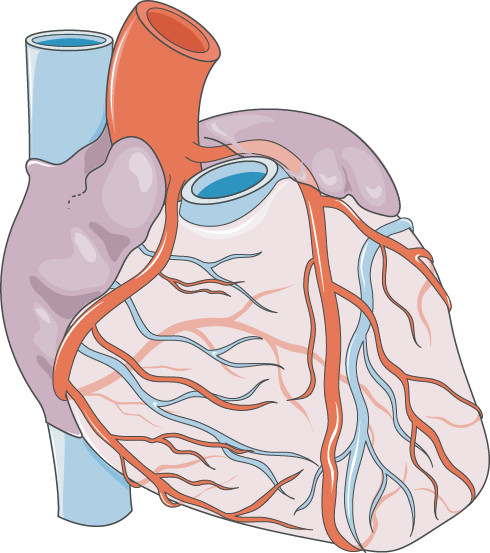
\includegraphics[width=0.34\textwidth]{servier-coronary-vessels.png}\\[3pt]
{\hei\footnotesize\color{hfslate} 心臟表面的冠狀動脈負責供應心肌的血流。}\\
{\itshape\scriptsize\color{hfslate} 插圖：Servier Medical Art（CC\,BY\,3.0）}
\end{center}

\tableofcontents

% =====================================================================
\mainmatter
% =====================================================================
\chapter{認識冠狀動脈與診斷}

\newthought{心臟就像一座永不停歇的幫浦}，將血液送往全身。而心臟肌肉本身的氧氣與養分，則是靠心臟表面三條主要的\textbf{冠狀動脈}供應——即左主幹冠狀動脈（再分出\textbf{左前降支 LAD}、\textbf{左迴旋支 LCx}）與\textbf{右冠狀動脈 RCA}。當這些血管變窄或阻塞，心肌便會「缺血」，出現胸悶、胸痛或喘等症狀。

\begin{figure*}[htbp]\centering
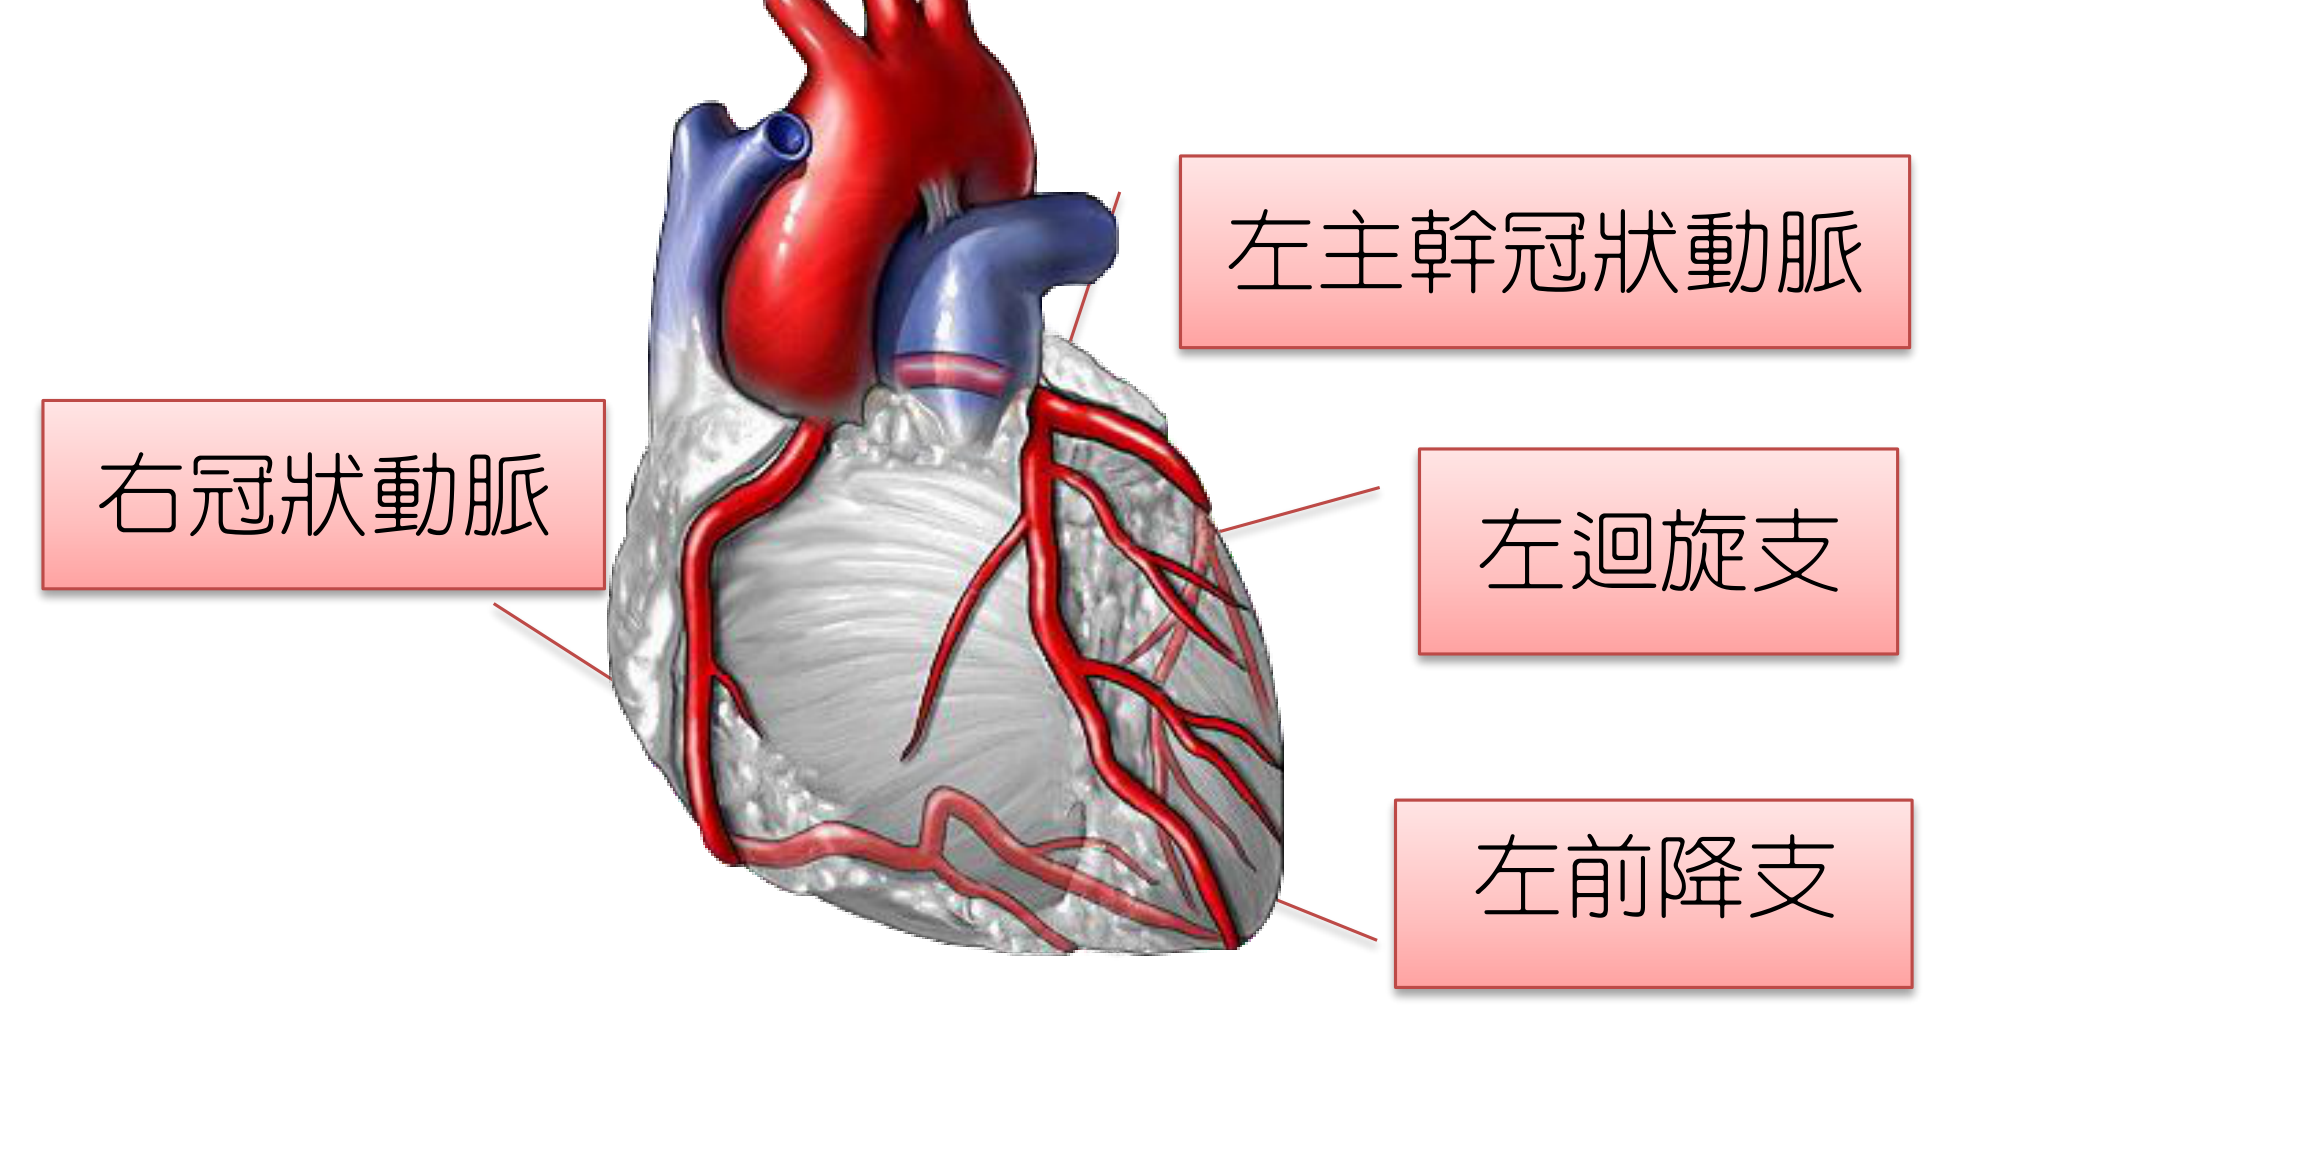
\includegraphics[width=0.86\linewidth]{coronary-anatomy.png}
\caption{\hei\small 心臟表面的三條主要冠狀動脈：左主幹冠狀動脈（分出左前降支、左迴旋支）與右冠狀動脈。}
\end{figure*}

\section{如何知道我的心臟血管有問題？}
當醫師懷疑冠狀動脈疾病時，可能安排\textbf{心電圖、運動心電圖、心臟超音波、核子醫學心肌灌注掃描}等非侵入性檢查評估。其中，\textbf{心導管冠狀動脈攝影}是目前診斷冠狀動脈狹窄最直接、最準確的檢查，能清楚看到狹窄的位置與嚴重程度。

\begin{figure*}[htb]\centering
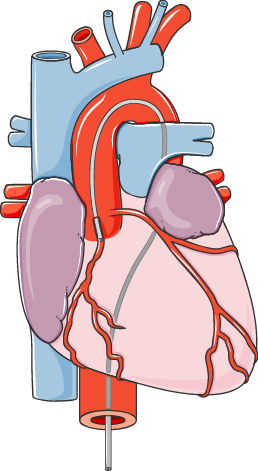
\includegraphics[width=0.24\textwidth]{servier-coronary-catheterization.png}
\caption{\hei\small 心導管檢查：將細導管從手腕或鼠蹊部送達心臟，進行冠狀動脈攝影。\quad{\itshape\scriptsize 插圖：Servier Medical Art（CC\,BY\,3.0）}}
\end{figure*}

\section{「狹窄超過 70\,\%」代表什麼？}
冠狀動脈攝影後，可直接判斷狹窄的部位與嚴重程度。\textbf{若血管狹窄超過 70\,\%}，心肌得到的血流明顯減少、氧氣供需失衡，可能造成胸悶、胸痛或活動時不適。\pearl{狹窄程度、位置、血管條數與心臟功能，都會影響治療方式的選擇——這也是為什麼需要和醫療團隊一起討論。}

\begin{figure*}[htbp]\centering
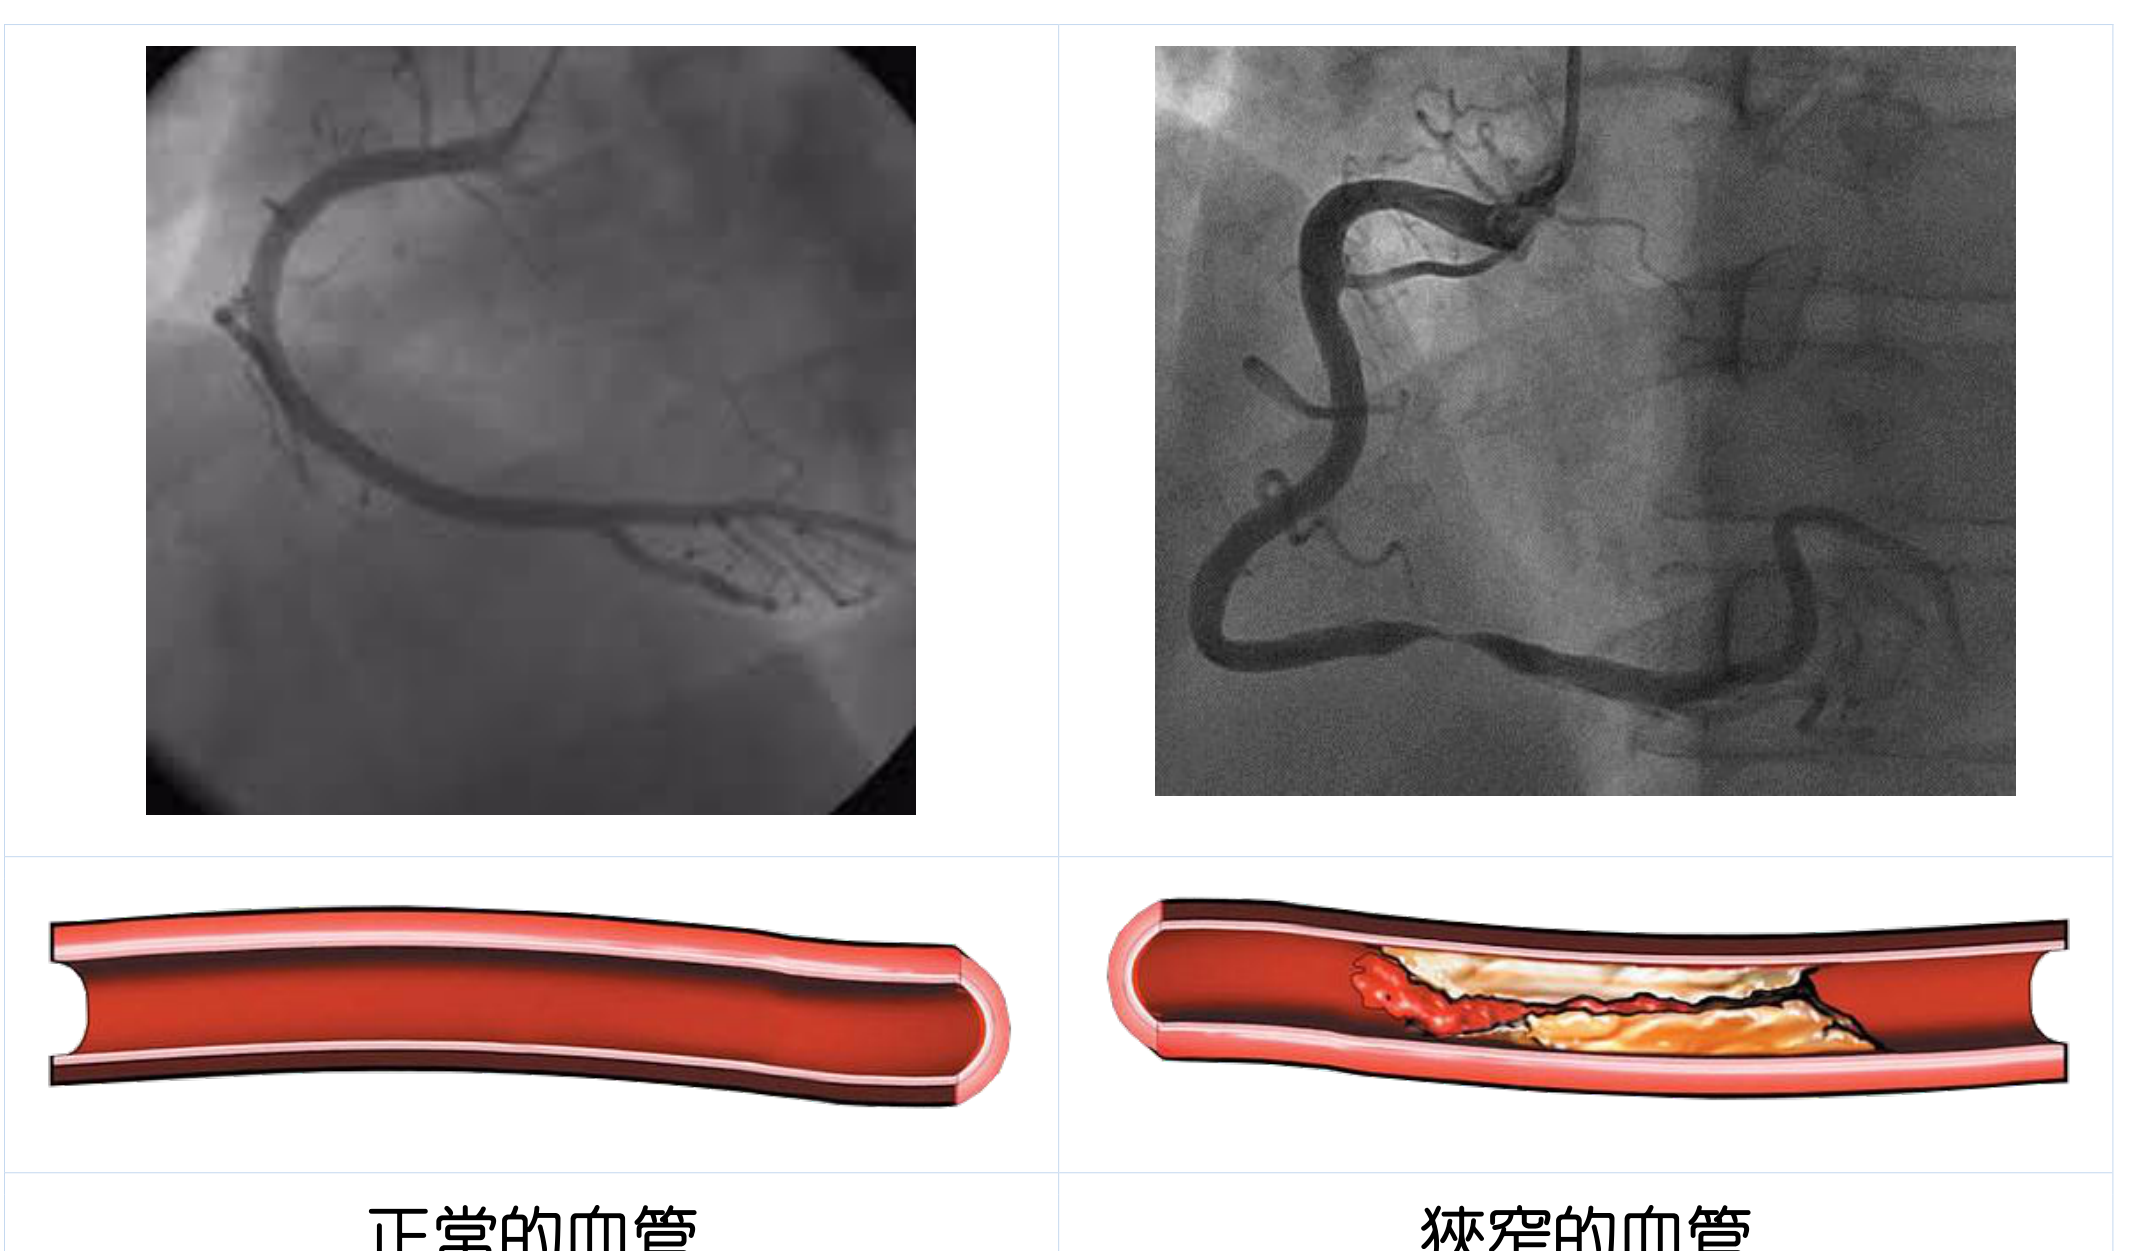
\includegraphics[width=\linewidth]{vessel-normal-vs-stenosis.png}
\caption{\hei\small 左為正常、暢通的血管；右為嚴重狹窄、堆積斑塊的血管。上排為冠狀動脈攝影影像，下排為血管剖面示意。}
\end{figure*}

% =====================================================================
\chapter{為什麼會有兩種選擇？}

\newthought{當冠狀動脈狹窄程度較輕}（約小於 70\,\%），通常可先以\textbf{調整生活型態與藥物治療}控制。但當血管出現\textbf{嚴重或重要部位的狹窄}，尤其已影響心臟功能時，就需要更積極處理。\defn{血流重建}{把狹窄、阻塞的血管重新打通或繞過，讓血流恢復供應心臟，醫學上稱為「血流重建（revascularization）」。}

根據醫學文獻與多數專家的共識，這時通常建議接受\textbf{心導管支架（PCI）}或\textbf{外科繞道手術（CABG）}。然而當檢查確定是\textbf{三條（含）以上血管嚴重狹窄}，或\textbf{左主幹}狹窄時，兩種方式往往都可行——這就是為什麼您會面臨「該選哪一種」的抉擇。

\begin{figure*}[htb]\centering
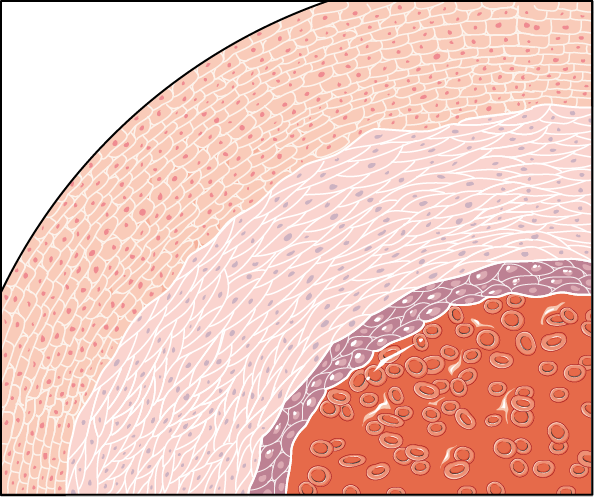
\includegraphics[width=0.42\textwidth]{servier-atherosclerosis.png}
\caption{\hei\small 動脈粥狀硬化：膽固醇等斑塊堆積在血管壁，使管腔逐漸變窄、血流受阻。\quad{\itshape\scriptsize 插圖：Laboratoires Servier（CC\,BY-SA\,3.0）}}
\end{figure*}

\begin{keybox}[沒有「絕對較好」，只有「比較適合」]
兩種治療都能達到血流重建的目的，\textbf{各有優缺點}。哪一種較適合，取決於您的血管條件、心臟功能、其他疾病、年齡、生活與工作型態，以及\textbf{您自己最在意的事}。
\end{keybox}

\section{首先，持續的藥物控制是共同的基礎}
不論最後選擇支架還是繞道手術，\textbf{規律服藥都不可或缺}。冠狀動脈疾病是慢性、會持續進展的疾病；手術或支架處理的是「目前最嚴重」的狹窄，但\textbf{保養血管、預防再狹窄與新病灶}，仍要靠長期藥物與生活控制。

\begin{keybox}[不論哪一種治療，都需要長期配合]
\begin{itemize}
\item \textbf{抗血小板藥物}（如阿斯匹靈、保栓通等）：預防血栓、保護支架或繞道血管暢通。
\item \textbf{降血脂（他汀類 statin）}：穩定斑塊、延緩動脈硬化進展。
\item \textbf{控制三高}：高血壓、高血糖、高血脂的良好控制。
\item \textbf{健康生活}：戒菸、規律運動、均衡飲食與心臟復健。
\end{itemize}
\textbf{請勿自行停藥}；任何用藥問題，請與您的醫療團隊討論。
\end{keybox}

% =====================================================================
\chapter{內科心導管支架（PCI）}

\newthought{內科心導管支架放置}（經皮冠狀動脈介入治療，PCI）是一種\textbf{侵入性較小}的治療方式。透過導管，從\textbf{手腕或鼠蹊部}的血管進入，送到心臟狹窄的冠狀動脈，先以氣球將狹窄處撐開，再放入\textbf{支架}支撐血管壁，讓血流恢復暢通。\defn{通常當天可完成}{多數情況下 PCI 為局部麻醉、傷口僅約 0.1～0.3 公分，是「微創、恢復快」的處置方式。}

\begin{figure*}[htbp]\centering
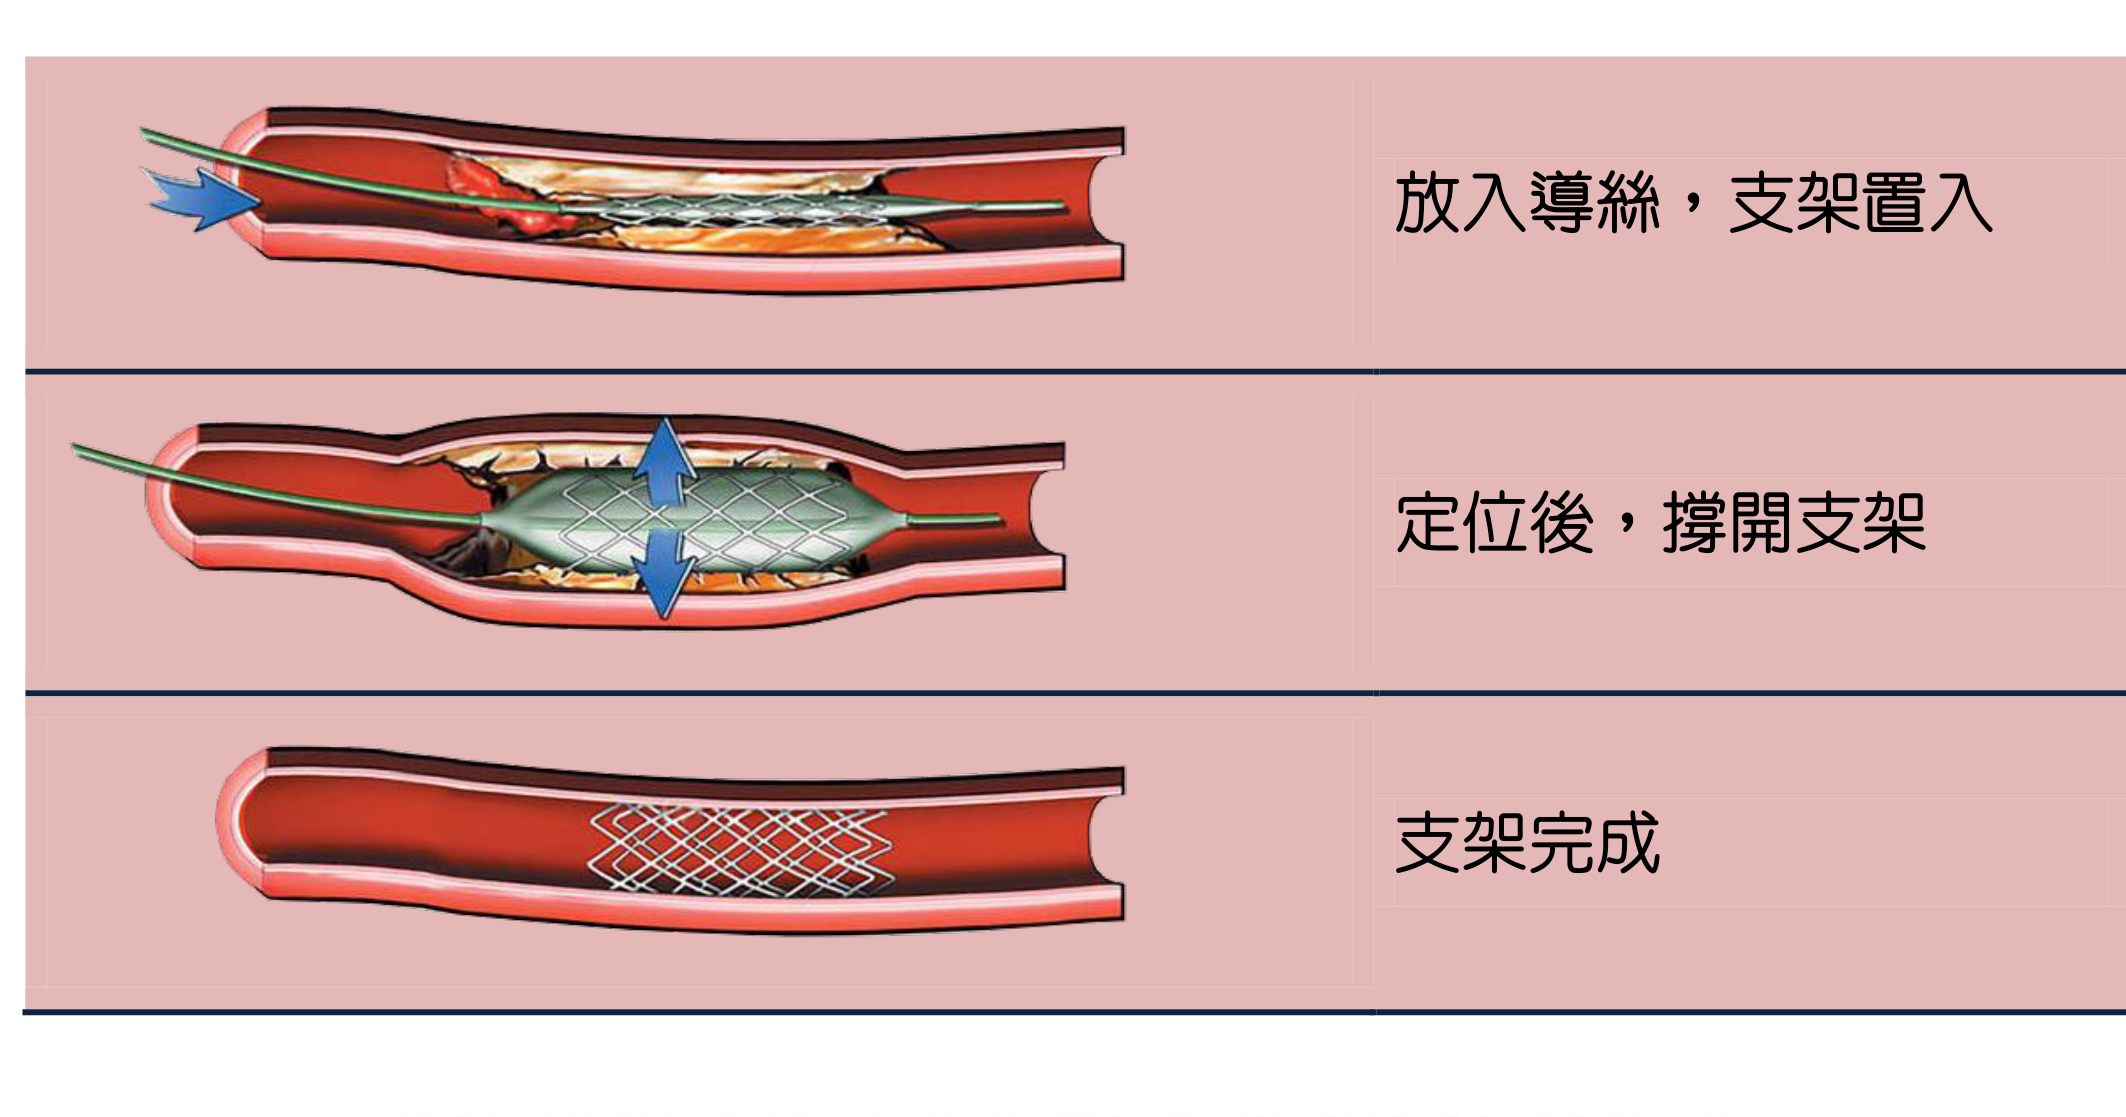
\includegraphics[width=\linewidth]{pci-stent-sequence.png}
\caption{\hei\small 支架置放的三個步驟：放入導絲與支架 → 定位後撐開支架（氣球擴張）→ 支架完成、撐住血管壁。}
\end{figure*}

\section{支架手術前後的樣子}
從冠狀動脈攝影影像可看到，\textbf{裝支架前}血管嚴重狹窄、血流受阻；\textbf{裝支架後}原本狹窄的血管被撐開，血流恢復暢通。

\begin{figure*}[htb]\centering
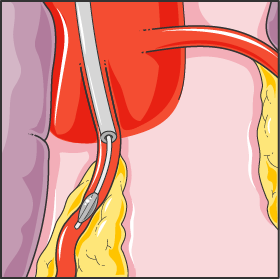
\includegraphics[width=0.34\textwidth]{servier-coronary-dilatation.png}
\caption{\hei\small 氣球擴張（血管成形術）將狹窄處撐開，再以支架支撐血管壁、維持血流暢通。\quad{\itshape\scriptsize 插圖：Laboratoires Servier（CC\,BY-SA\,3.0）}}
\end{figure*}

\begin{figure*}[htbp]\centering
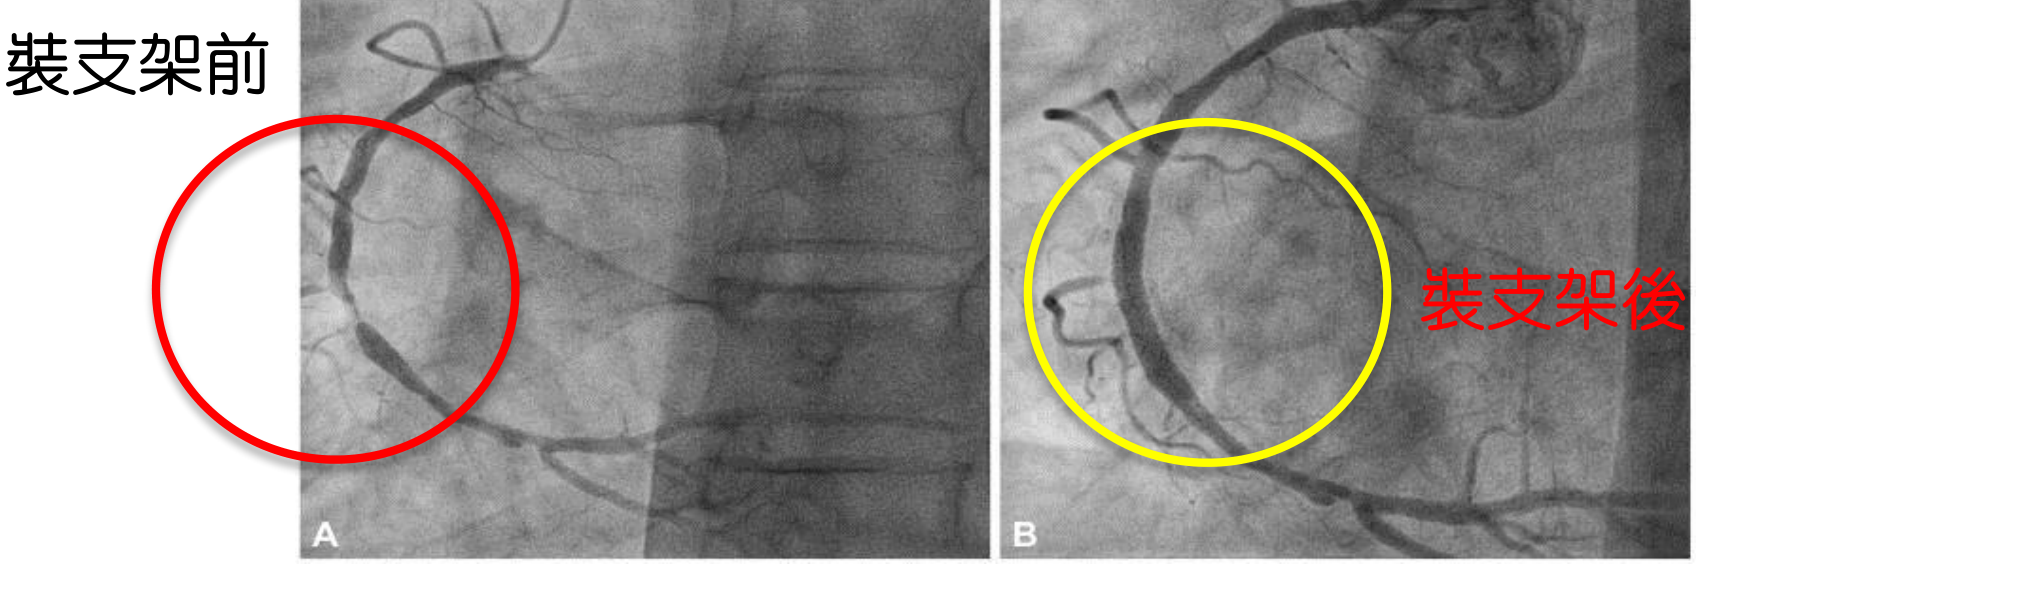
\includegraphics[width=\linewidth]{pci-before-after-angio.png}
\caption{\hei\small 裝支架前（紅圈，血管狹窄）與裝支架後（黃圈，血流恢復）的冠狀動脈攝影對照。}
\end{figure*}

\section{關於支架的種類}
目前臨床上多\textbf{建議使用「塗藥支架（DES）」}，能降低支架內再狹窄的機會。塗藥支架屬\textbf{自費}，費用約新台幣 15～20 萬元以上（視支架數量與材料而定，不含住院費用）。\pearl{放置支架後，\textbf{雙重抗血小板藥物}務必依醫囑按時服用、不可自行停藥，以免發生支架血栓。}

% =====================================================================
\chapter{外科冠狀動脈繞道手術（CABG）}

\newthought{冠狀動脈繞道手術}是利用病人\textbf{自身其他部位的血管}（例如腿部的大隱靜脈、胸壁的胸廓內乳動脈，或手臂的橈動脈），\textbf{繞過}心臟阻塞的部位，另造一條新的血流通道——就像在塞車的路段旁，開通一條新的道路。\defn{繞道用的血管}{常用的「橋血管」包括胸廓內乳動脈（IMA）、大隱靜脈與橈動脈，取自病人自己的身體。}

\begin{figure*}[htbp]\centering
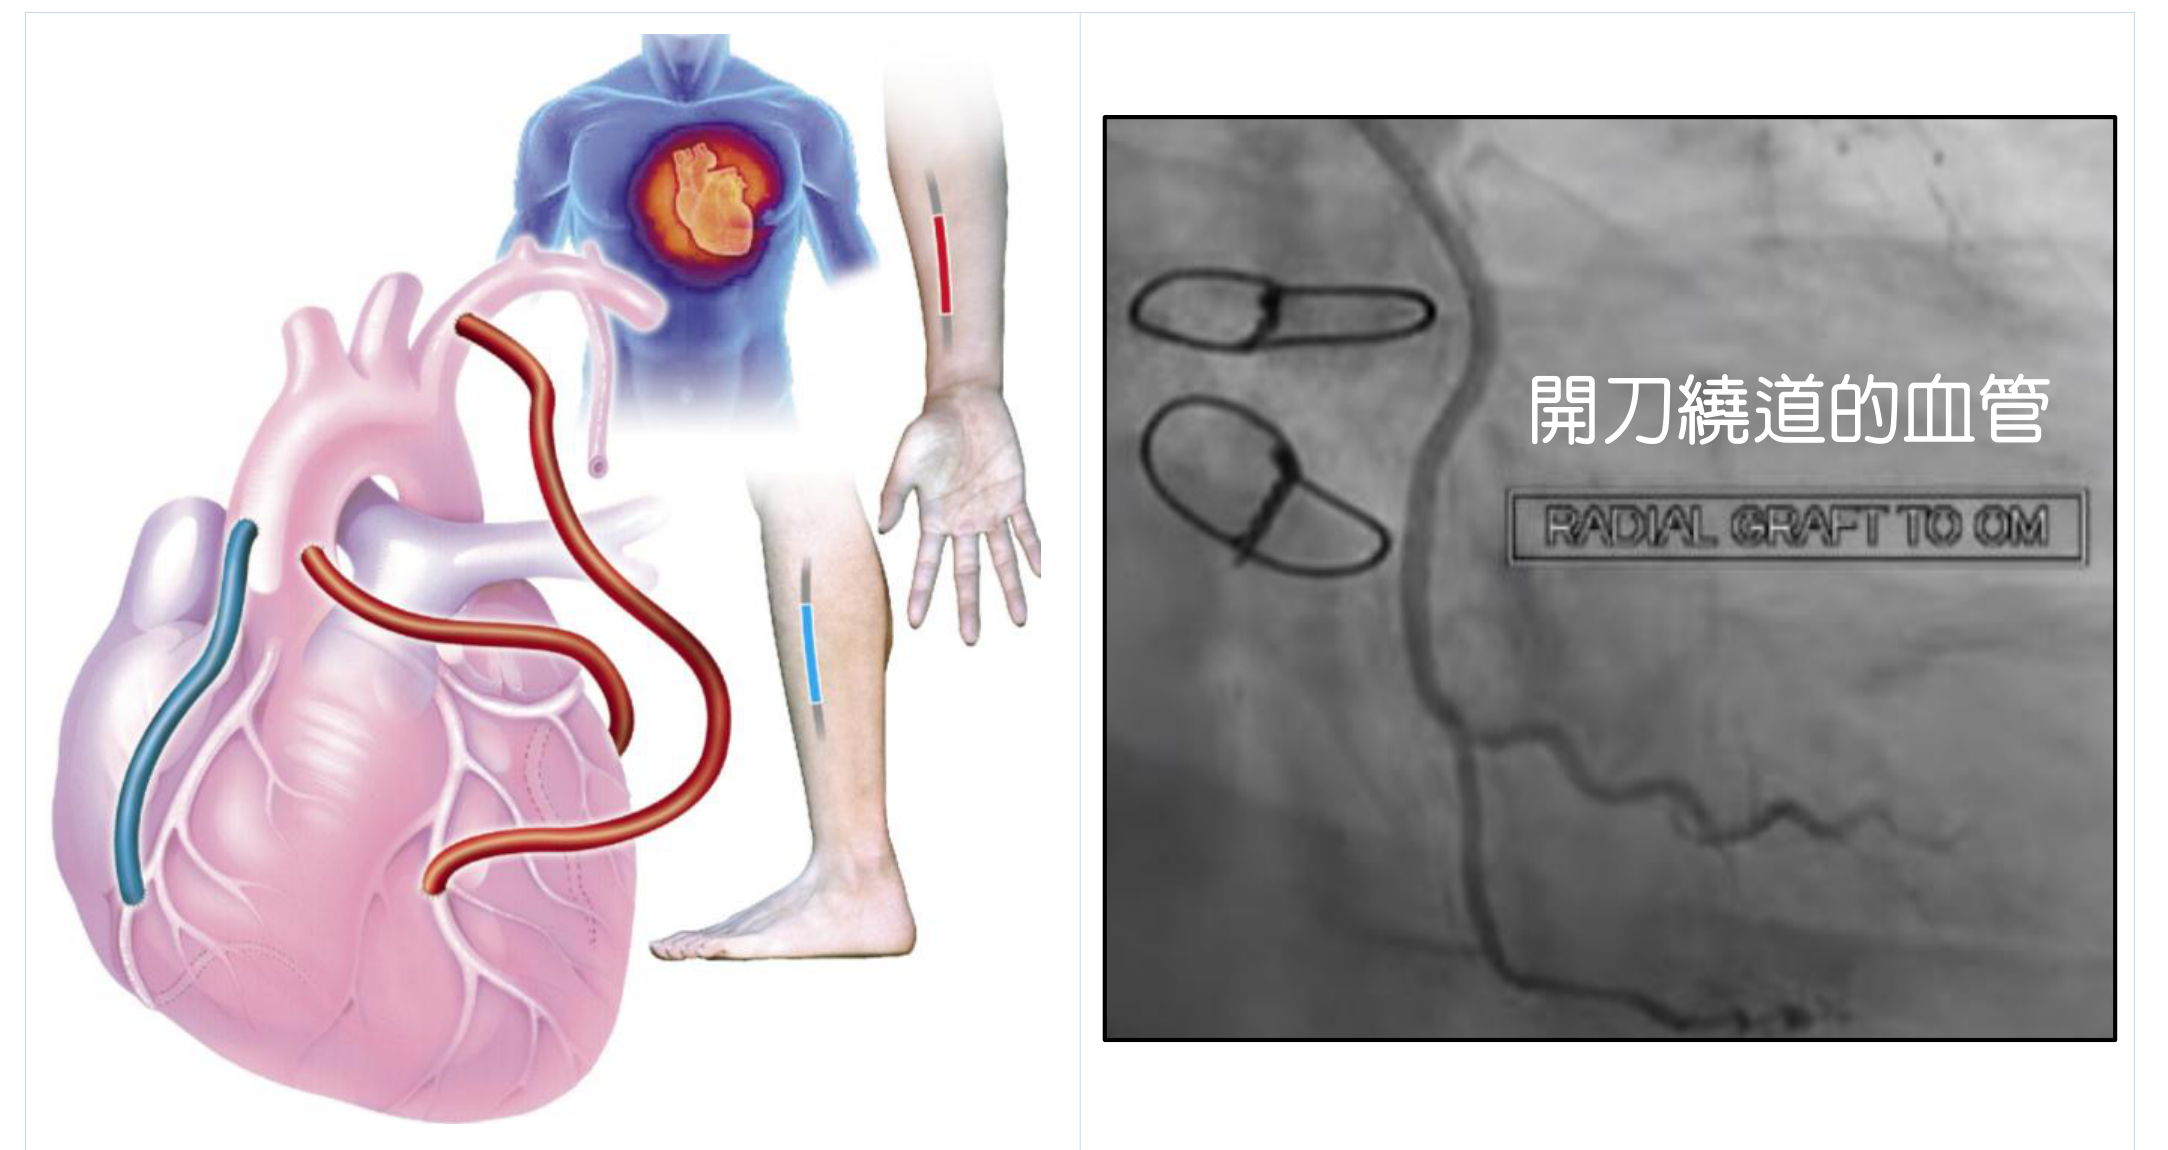
\includegraphics[width=\linewidth]{cabg-bypass.png}
\caption{\hei\small 左：以自身血管在阻塞處旁建立新的血流通道；中：橋血管來源（胸廓內乳動脈、橈動脈、大隱靜脈）；右：繞道後的血管攝影影像。}
\end{figure*}

\section{手術大致的過程}
繞道手術需\textbf{全身麻醉}。\textbf{傳統術式}傷口位於\textbf{胸部正中切口}，長度大約 15～20 公分；部分病人可採\textbf{微創術式}，傷口位於\textbf{左胸側邊}，長度大約 5～10 公分。手術時間約 4～6 小時（視情況而定），可\textbf{一次處理多條阻塞的血管}，達到較完整的血流重建。

\begin{figure*}[htb]\centering
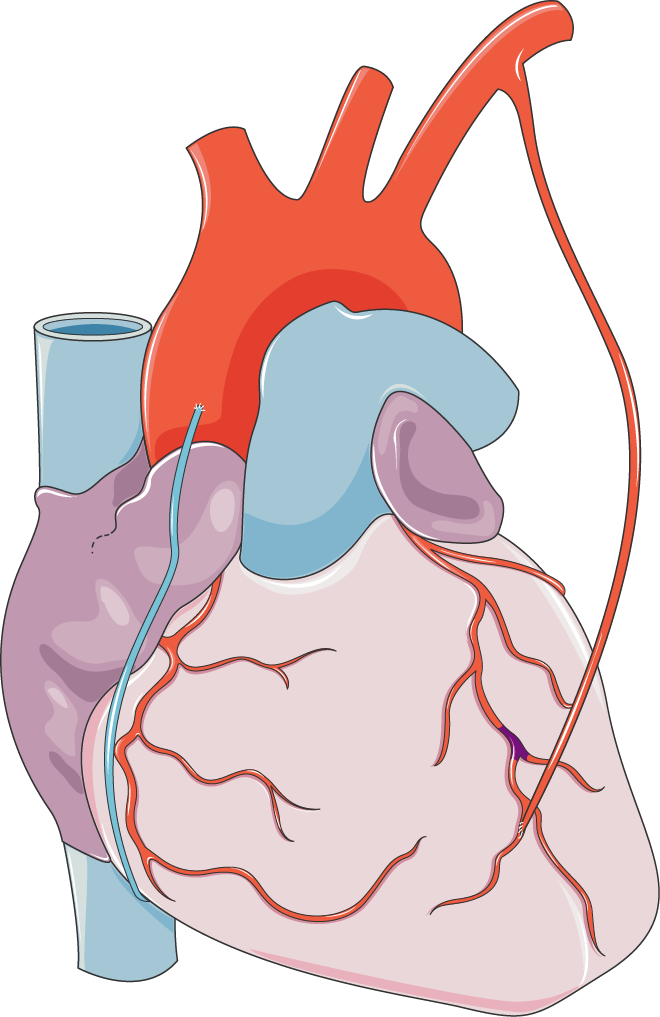
\includegraphics[width=0.26\textwidth]{servier-cabg.png}
\caption{\hei\small 繞道手術以自身的橋血管，繞過阻塞的血管段、在其下游重建血流。\quad{\itshape\scriptsize 插圖：Laboratoires Servier（CC\,BY-SA\,3.0）}}
\end{figure*}

\begin{keybox}[繞道手術的特點]
能\textbf{一次完整重建}多條血管的血流，\textbf{長期成效相對穩定持久}；對某些病例（如三條血管或左主幹病變、合併糖尿病等）甚至能提升存活率。相對地，它是較大的手術，\textbf{恢復期較長}，住院天數也較久。
\end{keybox}

% =====================================================================
\chapter{步驟一：兩種治療的比較}

下表逐項比較\textbf{心導管支架（PCI）}與\textbf{外科繞道手術（CABG）}。這些數字是\textbf{一般情況的參考}，您個人的狀況會因血管條件、心臟功能與其他疾病而不同，實際情形請與醫療團隊確認。

\begin{fullwidth}
\renewcommand{\arraystretch}{1.35}
\small\hei\color{hfslate}
\begin{tabular}{@{}>{\raggedright\arraybackslash}p{0.15\linewidth} >{\raggedright\arraybackslash}p{0.40\linewidth} >{\raggedright\arraybackslash}p{0.40\linewidth}@{}}
\toprule
\heibold\color{hfteal} 項目 & \heibold\color{pciblue} 內科心導管支架放置（PCI） & \heibold\color{hfred} 外科繞道手術（CABG）\\
\midrule
麻醉方式 & 局部麻醉。 & 全身麻醉。\\
傷口位置及大小 & 手腕或鼠蹊部，約 0.1～0.3 公分。 & 傳統手術：胸部正中切口，約 15～20 公分；微創手術：左側胸部切口，約 5～10 公分。\\
要拆線嗎 & 加壓止血，不需拆線。 & 需回診拆線。\\
手術時間 & 約 1.5～4 小時以上不等，視情況而定。 & 約 4～6 小時，視情況而定。\\
住院時間 & 約 3 天（加護病房 1～2 天，普通病房 1～2 天）。 & 約 10～14 天（加護病房 3～5 天，普通病房 7～8 天）。\\
一次解決嗎 & 不一定，有可能要多次施作。 & 一次完成。\\
風險（死亡率） & 心導管治療導致之死亡率平均約 \textbf{0.8～2.1\,\%}。 & 本院常規冠狀動脈繞道手術死亡率約 \textbf{1～3\,\%}。\\
長期比較 & 追蹤兩年，心血管不良事件（死亡、心肌梗塞再發、中風、再次接受導管治療等綜合發生率）約 \textbf{12.2\,\%}。 & 約 \textbf{8.1\,\%}。\\
費用 & 建議使用塗藥支架，支架及其他材料費\textbf{自費約 15～20 萬元以上}（不含住院費用）。 & \textbf{健保給付}，連同住院費用約 \textbf{10 萬元左右}。\\
\bottomrule
\end{tabular}
\renewcommand{\arraystretch}{1.0}
\end{fullwidth}

\srcnote{長期比較之實證主要來自 PRECOMBAT 試驗，詳見書末參考文獻。}

\section{各自的優點與缺點}
\begin{fullwidth}
\hei\color{hfslate}\small
\begin{tabular}{@{}>{\raggedright\arraybackslash}p{0.47\linewidth} >{\raggedright\arraybackslash}p{0.47\linewidth}@{}}
\toprule
\heibold\color{pciblue} 心導管支架（PCI） & \heibold\color{hfred} 外科繞道手術（CABG）\\
\midrule
\textbf{優點：}住院期與康復期較短；緩解症狀有效、恢復快；微創、傷口小，多為局部麻醉。
&
\textbf{優點：}能一次較完整重建多條血管；緩解症狀有效；對某些病例能提高存活率；長期效果相對穩定持久。
\\[6pt]
\textbf{缺點：}再狹窄發生率較繞道手術高；嚴重瀰漫性病變不一定能完全重建；長期效果相對不如繞道；日後仍有再次處置或手術的可能。
&
\textbf{缺點：}恢復期較長、住院天數較久；是較大的手術，需全身麻醉；第二次接受繞道手術的風險會比第一次高。
\\
\bottomrule
\end{tabular}
\end{fullwidth}

% =====================================================================
\chapter{步驟二：釐清我的價值與偏好}

請就以下每一句話，依您的\textbf{認同程度}打勾。\textbf{這份量表不計分、也不替您決定}——它的用意，是讓您想一想：對自己而言，哪些事最重要。某一份量表中您越認同的項目越多，代表那種治療\textbf{可能}較貼近您的期待；最終仍請與醫療團隊討論。

\bigskip
{\hei\large\color{hfteal} ① 我是不是應該選擇「外科繞道手術（CABG）」？}
\nopagebreak
\begin{fullwidth}
\renewcommand{\arraystretch}{1.6}
\hei\footnotesize\color{hfslate}
\begin{tabular}{@{}|>{\raggedright\arraybackslash}p{0.46\linewidth}|c|c|c|c|c|@{}}
\hline
\heibold 我的考量 & \heibold 不認同 & \heibold 不很認同 & \heibold 一般 & \heibold 認同 & \heibold 非常認同\\
\hline
我不用擔心復原期的問題，可以休養。 & & & & & \\ \hline
我很擔心醫療費用影響生活。 & & & & & \\ \hline
我想要一次在醫院就把所有的心臟血管處理好。 & & & & & \\ \hline
我知道三條血管狹窄，放支架和外科繞道手術風險差不多。 & & & & & \\ \hline
我想盡快回復正常運動型態。 & & & & & \\ \hline
我知道外科繞道手術的長期效果相對優於放置支架。 & & & & & \\ \hline
\end{tabular}
\renewcommand{\arraystretch}{1.0}
\end{fullwidth}

\bigskip
{\hei\large\color{pciblue} ② 我是不是應該選擇「內科心導管支架放置（PCI）」？}
\nopagebreak
\begin{fullwidth}
\renewcommand{\arraystretch}{1.6}
\hei\footnotesize\color{hfslate}
\begin{tabular}{@{}|>{\raggedright\arraybackslash}p{0.46\linewidth}|c|c|c|c|c|@{}}
\hline
\heibold 我的考量 & \heibold 不認同 & \heibold 不很認同 & \heibold 一般 & \heibold 認同 & \heibold 非常認同\\
\hline
我擔心恢復期很久。 & & & & & \\ \hline
我不太需要擔心醫療費用的問題。 & & & & & \\ \hline
三條以上的心臟血管狹窄問題，可以考慮分次長期進行。 & & & & & \\ \hline
我知道三條血管狹窄，放支架和外科繞道手術風險差不多。 & & & & & \\ \hline
我接受在心臟血管狹窄處置好前，運動型態將會受限。 & & & & & \\ \hline
我知道放置血管支架，可能會再反覆狹窄。 & & & & & \\ \hline
\end{tabular}
\renewcommand{\arraystretch}{1.0}
\end{fullwidth}

% =====================================================================
\chapter{步驟三：我的初步傾向}

把您在意的事再彙整一次。請就以下兩組個人考量，分別圈選「是」或「否」。哪一組您回答「是」的項目較多，\textbf{可能}就是目前較貼近您的選項。這只是幫助您整理想法，\textbf{不是最終決定}。

\bigskip
{\hei\large\color{hfred} ① 我打算選擇「外科繞道手術（CABG）」}
\nopagebreak
\begin{fullwidth}
\renewcommand{\arraystretch}{1.7}
\hei\small\color{hfslate}
\begin{tabular}{@{}|>{\raggedright\arraybackslash}p{0.66\linewidth}|c|c|@{}}
\hline
\heibold 我的考量 & \heibold 是 & \heibold 否\\
\hline
我知道要一段時間休養恢復。 & & \\ \hline
醫療費用比較低，我比較負擔得起。 & & \\ \hline
繞道手術可以幫我一次解決三條心臟血管的問題。 & & \\ \hline
我知道三條血管狹窄的情況下，放支架和外科繞道手術風險差不多。 & & \\ \hline
我想盡快回復正常生活及運動型態。 & & \\ \hline
我知道外科繞道手術的長期效果相對優於放置支架。 & & \\ \hline
\end{tabular}
\renewcommand{\arraystretch}{1.0}
\end{fullwidth}

\bigskip
{\hei\large\color{pciblue} ② 我打算選擇「內科心導管支架放置（PCI）」}
\nopagebreak
\begin{fullwidth}
\renewcommand{\arraystretch}{1.7}
\hei\small\color{hfslate}
\begin{tabular}{@{}|>{\raggedright\arraybackslash}p{0.66\linewidth}|c|c|@{}}
\hline
\heibold 我的考量 & \heibold 是 & \heibold 否\\
\hline
住院天數短，恢復期很快。 & & \\ \hline
我不太擔心醫療費用，不影響家庭支出。 & & \\ \hline
我知道處理三條以上的血管狹窄可能會分多次進行，沒辦法一次完成。 & & \\ \hline
我知道三條血管狹窄放支架和外科繞道手術風險差不多。 & & \\ \hline
我知道在心臟血管狹窄處置好前，生活和運動型態將會受限。 & & \\ \hline
我知道放置血管支架可能會再反覆狹窄。 & & \\ \hline
\end{tabular}
\renewcommand{\arraystretch}{1.0}
\end{fullwidth}

% =====================================================================
\chapter{步驟四：我準備好了嗎？}

經過前面幾個步驟，您已花了一些時間了解「外科繞道手術（CABG）」與「內科心導管支架放置（PCI）」的差異，也想過一些會影響決定的因素。現在，請檢視一下自己的準備狀態——\textbf{不論結果如何，都沒有對錯}。

\bigskip
\hei\color{hfslate}
\textbf{1. 我清楚知道有哪些治療的選擇。}\par
\quad \tick\ 知道 \qquad \tick\ 還不太清楚\par
\medskip
\textbf{2. 我已經接受足夠的資訊與建議，可以做決定。}\par
\quad \tick\ 是 \qquad \tick\ 否\par
\medskip

\begin{keybox}[3. 我已經確認想要的治療方式，我決定選擇：]
\tick\ 外科繞道手術（CABG）\par
\tick\ 內科心導管支架放置（PCI）\par
\tick\ 我還需要再考慮，尚未決定\rule[-2pt]{0.45\linewidth}{0.4pt}
\end{keybox}

\hei\color{hfslate}
\textbf{4. 還有什麼想法？}（可複選）\par
\quad \tick\ 我想要再更深入了解每一種治療方式。\par
\quad \tick\ 我需要再和家人、朋友或醫師討論看看。\par
\quad \tick\ 不用了，我已經做好我的選擇。\par

\bigskip
\begin{keybox}[還有疑問嗎？我們在這裡陪您]
完成以上內容後，若您還有任何不確定，都沒有關係。\\[3pt]
歡迎您\heibold\color{hfred}回到心臟內科或心臟外科門診\normalfont\hei\color{hfslate}，與您的主治醫師當面討論，一起選擇最適合您的治療方式。
\end{keybox}

% =====================================================================
\backmatter
\chapter{參考文獻與製作團隊}

\section*{實證依據}
左主幹／多條血管病變之支架（PCI）與繞道手術（CABG）長期成效比較，主要實證來自 \textbf{PRECOMBAT} 隨機分派試驗：
\begin{enumerate}[leftmargin=1.8em]
\item Park SJ, Kim YH, Park DW, Yun SC, Ahn JM, Song HG, et al. Randomized trial of stents versus bypass surgery for left main coronary artery disease. \textit{N Engl J Med.} 2011;364(18):1718–27.
\item Park DW, Ahn JM, Park H, Yun SC, Kang DY, Lee PH, et al. Ten-Year Outcomes After Drug-Eluting Stents Versus Coronary Artery Bypass Grafting for Left Main Coronary Disease: Extended Follow-Up of the PRECOMBAT Trial. \textit{Circulation.} 2020;141(18):1437–46.
\end{enumerate}

\noindent{\footnotesize\hei\color{hfslate} 本工具之比較數據與費用，引自新竹臺大分院心血管中心原醫病共享決策衛教資料（2020 年第一版）；實際數字會因個人病情、術式與健保給付規定而調整，請以醫療團隊說明為準。}

\section*{圖片來源與授權}
標示「Servier Medical Art」的醫學插圖，來自 Servier Medical Art（Laboratoires Servier，\texttt{smart.servier.com}），經 Wikimedia Commons 取得，依 Creative Commons 授權使用（僅縮放、未修改內容）：
\begin{itemize}
\item 心臟與冠狀動脈、心導管檢查 —— Servier Medical Art，授權 CC\,BY\,3.0。
\item 動脈粥狀硬化、氣球擴張與支架、冠狀動脈繞道手術 —— Laboratoires Servier，授權 CC\,BY-SA\,3.0。
\end{itemize}
\noindent{\footnotesize\hei\color{hfslate} 其餘解剖圖、心導管攝影與手術示意圖，取自新竹臺大分院心血管中心原醫病共享決策衛教資料。}

\vspace{2em}
\begin{fullwidth}\centering
{\heibold\color{hfteal} 製作團隊}\\[8pt]
{\hei\small\color{hfslate}
國立臺灣大學醫學院附設醫院新竹臺大分院　心導管室\\[4pt]
謝明倩　放射師（心導管室組長）}\\[12pt]
{\hei\footnotesize\color{hfslate} 新竹臺大分院　心血管中心　醫病共享決策　·　2020 年第一版／2026 年 Tufte 版重新編修}
\end{fullwidth}

\end{document}
